
%(BEGIN_QUESTION)
% Copyright 2012, Tony R. Kuphaldt, released under the Creative Commons Attribution License (v 1.0)
% This means you may do almost anything with this work of mine, so long as you give me proper credit

Suppose a FOUNDATION Fieldbus temperature transmitter will be used to measure how close the liquid inside a vessel approaches the boiling point of water (212 degrees Fahrenheit).  The transmitter senses temperature using an RTD sensor over an expected range of 40 $^{o}$F to 200 $^{o}$F, but we wish the operations personnel to see a temperature display ranging from -172 to -12 (the number of degrees below the boiling point of 212 $^{o}$F).

$$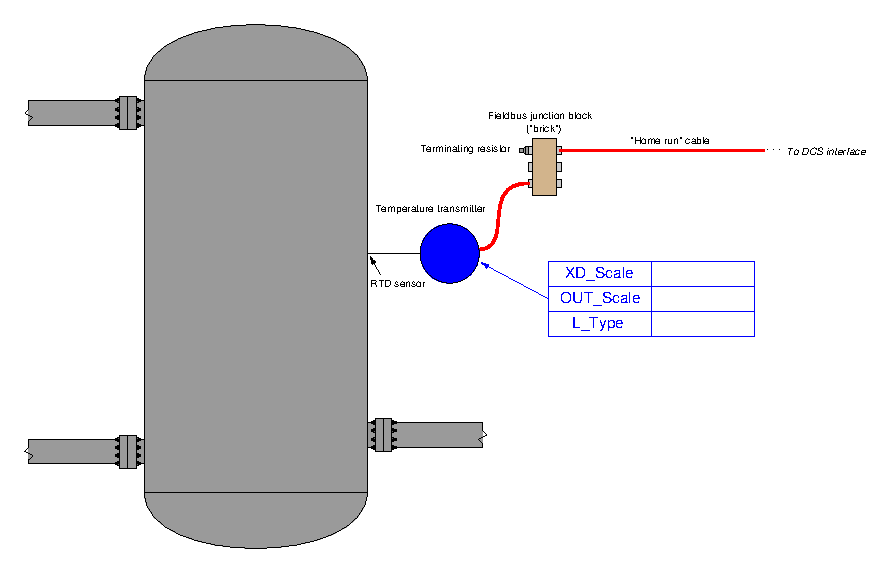
\includegraphics[width=15.5cm]{i04719x01.eps}$$

Complete the configuration table in the above illustration, showing the proper {\tt XD\_Scale}, {\tt OUT\_Scale}, and {\tt L\_Type} parameter values to make the transmitter function as it should in this application.

\vskip 20pt \vbox{\hrule \hbox{\strut \vrule{} {\bf Suggestions for Socratic discussion} \vrule} \hrule}

\begin{itemize}
\item{} If the {\tt XD\_Scale} were set to a range of 40 to 212 degrees and the {\tt OUT\_Scale} set to a range of -172 to 0 degrees, would it work for this application?  Explain why or why not.
\end{itemize}

\underbar{file i04719}
%(END_QUESTION)





%(BEGIN_ANSWER)

{\tt XD\_Scale} = 40 to 200 degrees Fahrenheit

\vskip 10pt

{\tt OUT\_Scale} = -172 to -12 degrees (below boiling)

\vskip 10pt

{\tt L\_Type} = Indirect

%(END_ANSWER)





%(BEGIN_NOTES)


%INDEX% Fieldbus, instrument ranging: setting XD_Scale and OUT_Scale parameters for an application

%(END_NOTES)

